\chapter{Lexicalized domain representations and Sparse layers}
\label{chap:ldr}
\section{Introduction}
In this chapter, we present an MDMT system that we developed and published in \citet{Pham19generic}. Our system "Lexicalized domain representation" (LDR \nomenclature[ldr]{LDR}{Lexicalized domain representation}) was introduced in Section ~\ref{ssec:systems-chap4} of the previous chapter and used as an MDMT baseline in our overview. Recently, we extended the idea of LDR, in which a number of units in the $0^{th}$ layer are reserved for one domain and are dropped when translating in other domains to Sparse layers, in which not only the $0^{th}$ layer but also higher layers use the same dropping mechanism.

The \emph{supervised multi-domain adaptation} setting presented in Section \ref{sec:case1} usually involves a large number of domains. Adapting the whole NMT system separately to each domain would waste training resources and require large hardware resources for maintenance. We develop a simple MDMT system that changes only the form of word embeddings, i.e., can be applied to any NMT architecture. Our proposal transposes to neural machine translation the feature expansion technique of (Daum\'e III, 2007). We isolate domain-agnostic from domain-specific units in word embeddings while sharing the rest of the network across domains. Our main hypothesis is that domains mostly differ at the lexical level due to cross-domain polysemy, which motivates domain-specific embeddings. Another motivation to reconstruct only word embeddings is that we can easily handle the growing number of domains by creating more domain-specific units, which can not be done so easily in higher layers.

Sparse layers are extensions of LDRs in higher levels of an NMT model. These layers create a partition of nodes in the network of an NMT model assigning different sub-networks to different domains. By doing this, we reduce the interference between domains in the contribution of the parameters to the prediction. Our first version of Sparse layers is hard-coded, i.e., the choice of dropping mask is heuristically predefined. However, the dropping pattern can be learned via a latent variable \citet{Gong21pay,Gong21adaptive}.
 
Our experiments are complementary to those in Chapter ~\ref{chap:revisiting} and consider four domains, two neural architectures, and two language pairs and find that our technique yields effective multi-domain NMTs, outperforming several baselines. We also report the performance of \system{LDR} in a highly heterogeneous MDMT setting (see Chapter ~\ref{chap:revisiting}). We evaluate Sparse layers in the same MDMT setting as in Chapter ~\ref{chap:revisiting}.

Our contributions are thus as follows: we adapt and implement the ideas of \citet{Daume07frustratingly} for two NMT architectures; we provide experimental evidence that shows the effectiveness of this technique; we evaluate the ability of our networks to accommodate new domains dynamically; we apply the idea of the sparse representation from \system{LDR} to higher layers and receive promising results in a highly heterogeneous MDMT setting. Finally, we introduce a new technique to analyze word polysemy using embeddings, which comforts the assumption that their variation across domains reflects the change of senses.

\section{Lexicalized domain representations\label{sec:lexicalized_embeddings-chap5}}
\subsection{Multi-domain machine translation \label{ssec:statement-chap5}}
As introduced in Section ~\ref{ssec:4cases-chap3}, a train example in the \emph{supervised multi-domain adaptation} setting is a triplet $(d,x,y)$, with $x$ in the source language, $y$ in the target language and $d$ a domain tag in $[1\dots n_d]$. According to Section ~\ref{ssec:formulizaion} the training instances are distributed according to a mixture $\mathcal{D}_e^S$ such that $\mathcal{D}_e^S(x) = \sum_{d=1}^{n_d} \lambda^{s}(d) \mathcal{D}_e^d(x)$, with $\{\lambda^{s}(d), d=1 \dots n_d\}$ the mixture weights satisfying $\sum_d \lambda^{s}(d)=1$. According to our definition of the NMT loss function in Equation ~\eqref{eq:ce-chap2} and our definition of multi-domain distribution in Section ~\ref{ssec:formulizaion} and Section ~\ref{sec:domain}, our objective is to find a tuple of parameters $\{\theta_1 \dots \theta_d \} \in \mathbb{R}^D \times \dots \times \mathbb{R}^D$ minimizing:
\begin{equation} \label{eq:loss-chap5}
\begin{split}
\sum_{d \in [1..n_d]} \lambda^{s}(d) E_{x \sim \mathcal{D}_e^d(x), y \sim g^d(x)} [-log(P(y|x,\theta_d))] \text{.}
\end{split}
\end{equation}
in which the labeling function of each domain $d$ will be $g^d: \Omega_{e} \rightarrow \Omega_{f}$ where $\Omega_{e}$ and $\Omega_{f}$ are the set of sentences in the language $e$ and the language $f$ respectively.

A straightforward solution is to process each domain separately, computing the value $\theta_d^*$ that minimizes the empirical loss in $\mathcal{D}_e^d$ and $g^d$. This strategy is only effective if we have sufficient training data for each domain; when this is not the case, some estimates $\theta_d^*$ may be far from their optimal value. The alternative we consider here constraints each parameter $\theta_d$ to be made of two parts: $\theta_d = [\theta_s; \theta'_d]$. $\theta_s \in R^{D_g}$ is shared across all domains, while the second part $\theta'_d \in \mathbb{R}^{D_d}$ is only used in domain $d$.
The parameter set is much more constrained, yet we expect that tying parameters across domains will yield better estimates for $\theta_s$ due to a larger training corpus. In this setting, the optimization program defined by equation~\eqref{eq:loss-chap5} can no longer be performed separately for each training corpus.

\subsection{Lexicalized domain embeddings \label{ssec:lde-chap5}}
To actually implement this idea for NMT, we need to define the subset of parameters that will be shared across domains. In this section, we explore the hypothesis that domain specificities can be confined to the lexical level, and we define $\theta_s$ to contain all the network parameters except for a subpart of the word embeddings. 
For each word $v$, the embedding vector $e(v)$ is thus decomposed as $e(v) = [e_g(v); e_1(v); \dots; e_d(v)]$, where $e_g(v)$ stores the domain-agnostic lexical embedding, while $e_d(v)$ stores the subpart that is specific to domain $d$.
In our NMT architectures, the actual embedding layer composes these vectors linearly to generate the word embedding for domain $k$ according to:

\begin{align}
  \tilde{e}_k(v) =& M_g e_g(v) + \sum_{d \in [1,..,n_d]} M_d \times e_d(v) \times \delta(d=k) \nonumber \\
   & = M [e_g(v); e_1'(v,k) \dots; e_d'(v,k)], \label{eq:embedding-chap5}
\end{align}
where $\delta()$ is the indicator function, $M$ is the matrix made of blocks $M_g, M_1 \dots, M_{n_d}$, and $e_d'(v,k)$ is the masked embedding: $e_d'(v,k)= e_d(v) * \delta(d=k)$.  

\begin{figure}[h!]
  \center
  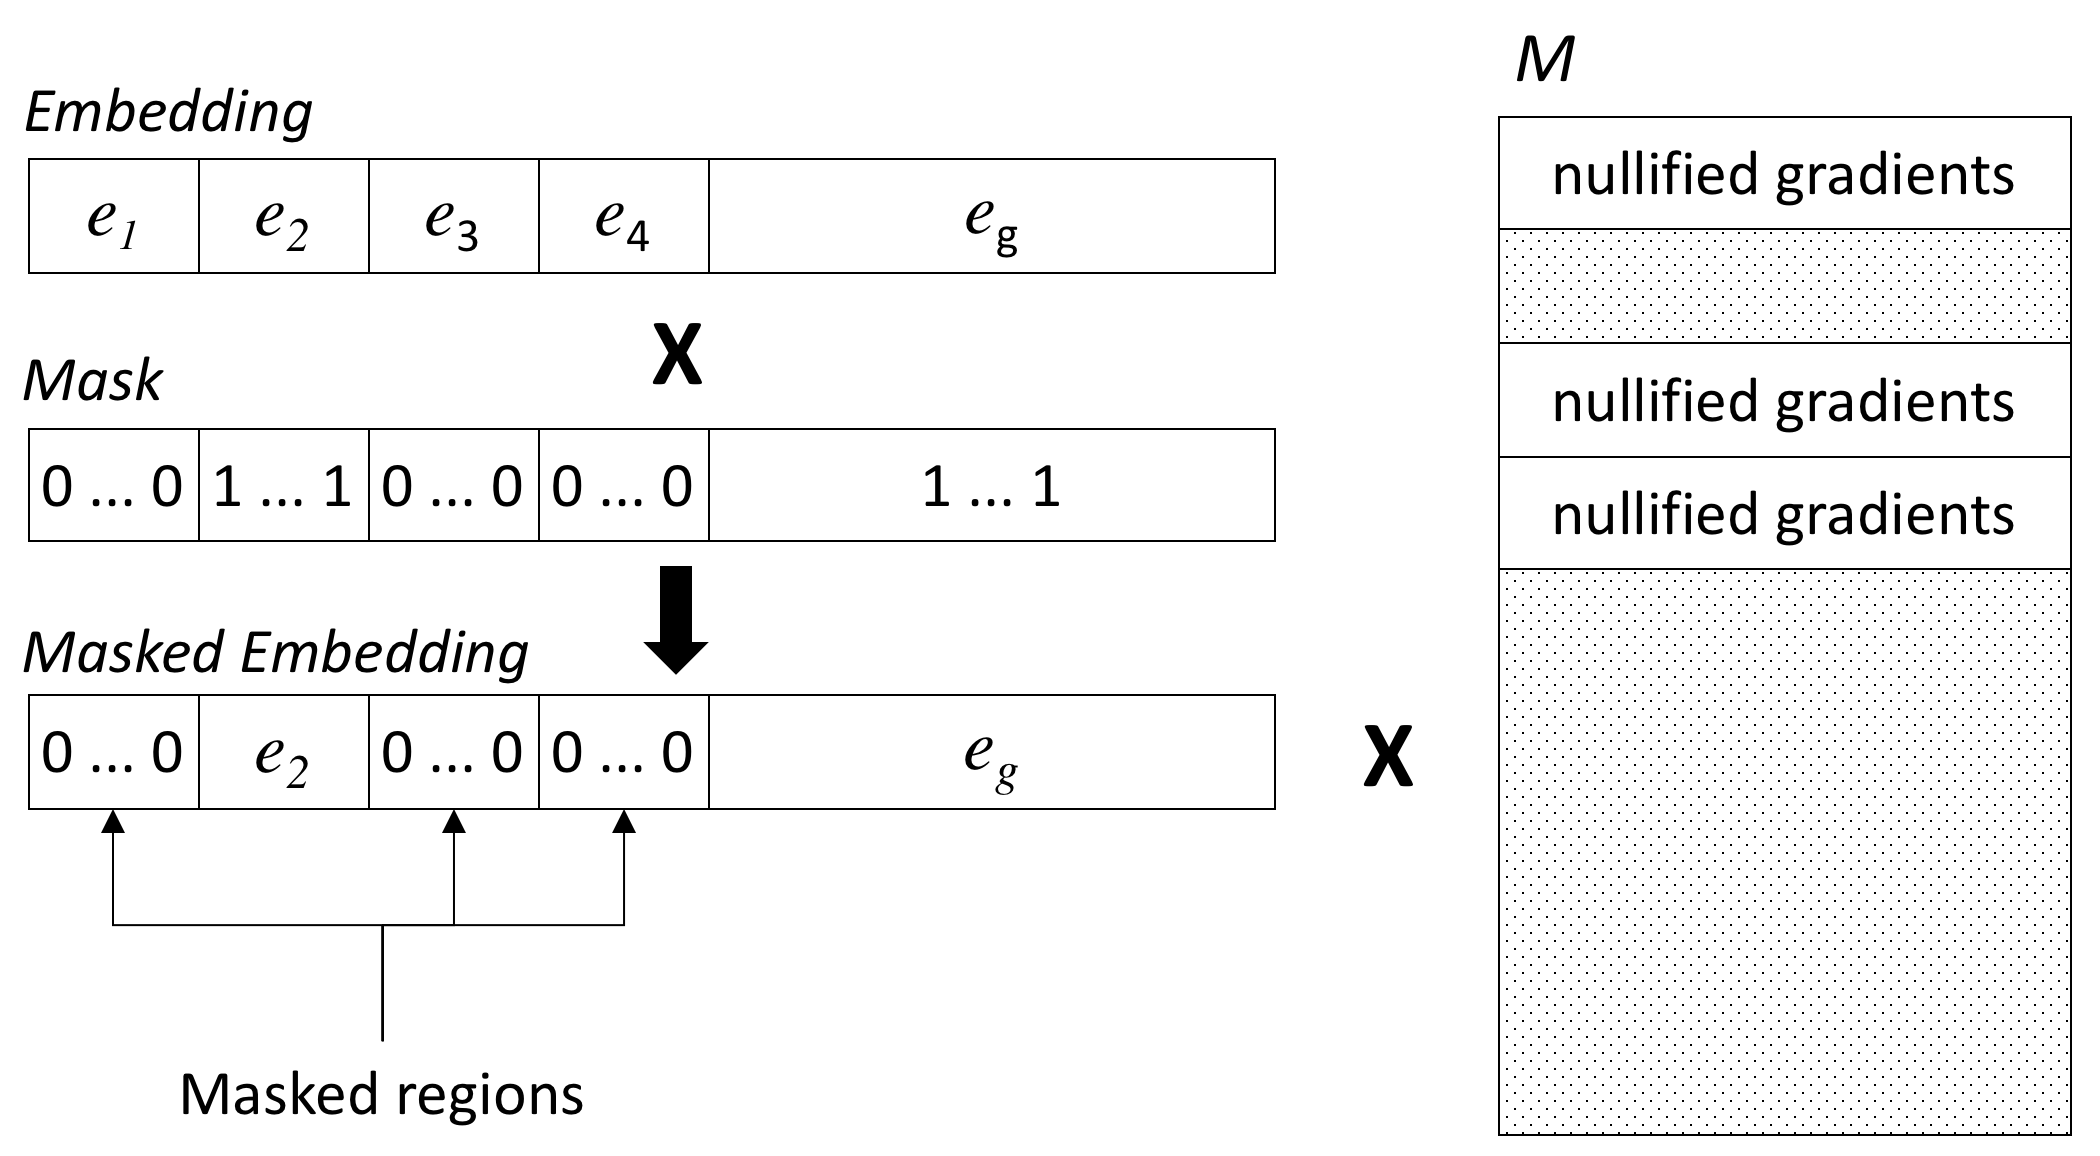
\includegraphics[width=0.6\textwidth]{graphics/embeddings}
  \caption{Lexicalized domain embeddings. When processing a sample from domain $2$, we only activate the corresponding parameter region ($\theta_2$) in the input embeddings; the remaining domain-specific parts are zeroed out and do not receive any update. The domain-agnostic part is always active and is updated irrespective of the input domain.} 
  \label{fig:network-chap5}
\end{figure}

Ensuring that the actual embedding does not contain any zero is essential for the Transformer model since the lexical representations are added to the positional encoding, which would undo the effect of domain masking and propagate a gradient even to regions that should not be modified. With our design, we make sure that the matrix $M$ receives gradient $0$ at regions corresponding to deactivated regions in the word embedding during backpropagation. Those regions are also masked in the forward step. Thus they do not interfere with the training on the domains to which they are not assigned (see Figure~\ref{fig:network-chap5}). Our architecture is thus readily compatible with any NMT architecture, where we replace standard embedding layers with the embeddings defined in equation~\eqref{eq:embedding-chap5}. In our experiments, we consider both the attentional RNN architecture of \citet{Bahdanau15learning} and the Transformer architecture of \citet{Vaswani17attention}.

\section{Sparse layers}
\label{sec:sparse-chap5}
Sparse layers replace the linear combination of domain-agnostic units and domain-specific units used to compute LDR embeddings by multiplying the output of each layer with domain-specific dropping vector as follows

\begin{equation}
\begin{array}{rcl}
\tilde{h}^{l} &=& h^{l} * r^{l}(d) \\
r^{l}(d) & \in & \mathbb{R}^{d_k} \\
r^{l}(d)_i &=& \begin{cases}
      1, & \text{if}\ i<d_a \\
      1, & \text{if}\ d_a + d \times \frac{d_k - d_a}{n_d} <= i < d_a + (d+1) \times \frac{d_k - d_a}{n_d} \\
      0, & \text{otherwise}
    \end{cases} \\
d & \in & \{0,\dots,n_d-1 \} \\
\end{array}
\label{eq:sparse-chap5}
\end{equation}
$h_l$ is the output of the $l^{th}$ layer; $d_a$ is the number of domain-agnostic nodes; $n_d$ is the number of domains. We allocate the same number of domain-specific nodes for every domain. However, the number of nodes in each intermediate layer is always fixed at $d_k$, \system{Sparse} layers can not dynamically create more units for new domains. Therefore, the model currently only handles a fixed number of domains. In Section ~\ref{sec:conclusion-chap5} we will discuss a promising approach that allows \system{Sparse} to handle an arbitrary number of domains.

\begin{figure}[h!]
  \center
  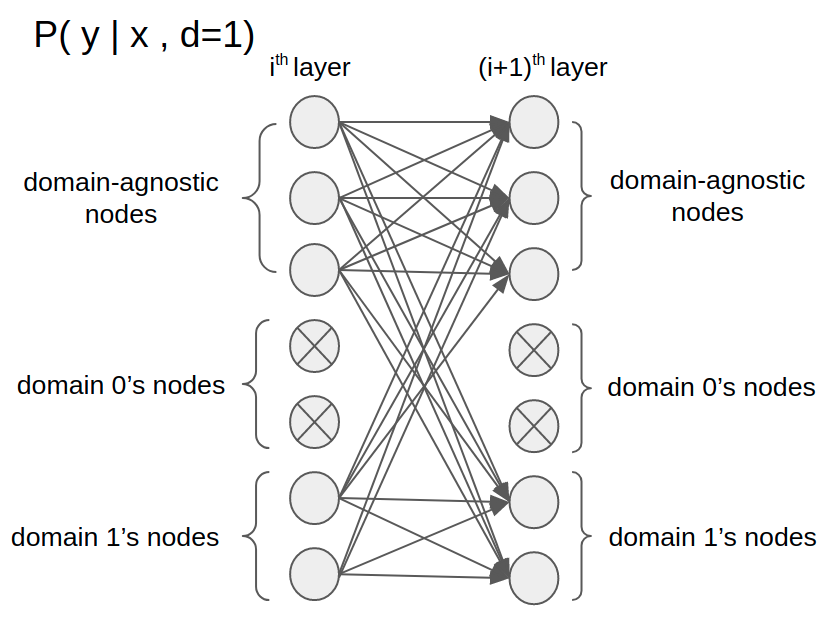
\includegraphics[width=0.6\textwidth]{graphics/Sparse_layers}
  \caption{Sparse layers. When processing a sample from domain $1$, only the signal of the domain-agnostic nodes and the $1^{th}$ domain's nodes are passed to higher layers, other nodes are dropped out.} 
  \label{fig:sparse-chap5}
\end{figure}
In our experiments with \system{Sparse}, we consider only the Transformer architecture of \citet{Vaswani17attention} and the same experimental setting as in Section ~\ref{ssec:corpora-chap4}.

\section{Experiments \label{sec:experiments-chap5}}
\subsection{Domains, data and metrics \label{ssec:data-chap5}}
\subsubsection{4 domains, 2 language pairs}
We experiment with two language pairs (English-French, English-German) and data originating from three domains, corresponding to texts from three European institutions: 
the European Parlement (EPPS) \citep{Koehn05europarl}, 
the European Medicines Agency (EMEA), 
the European Central Bank (ECB) \citep{Tiedemann09news},
In addition, for English-French we also use corpora in the IT-domain obtained from the OPUS web site\footnote{\url{http://opus.nlpl.eu}} corresponding to KDE, Ubuntu, GNOME and PHP datasets (IT). Moreover, we use IT only in the scenario of continual training, in which we continue training our MDMT system with the mix of new domain IT and the old domains EMEA, ECB and EPPS.

We randomly split those corpora into training, validation and test sets (see statistics in Table~\ref{tab:Corpora-chap5}).
Validation sets are used to chose the best model according to the average BLEU score \citep{Papineni02bleu}\footnote{We use detokenized truecasing multibleu.}

\begin{table}[h]
  \centering
  \begin{tabular}{ |llll|} %*{4}{|r|}}
    \hline
    Corpus & Train & Valid & Test \\ 
    \hline
    \multicolumn{4}{l}{English $\rightarrow$ French }\\
    %\multicolumn{4}{|l|}{Vocab size - En: 30,165, Fr: 30,398}\\
    \hline
    EMEA  & 1.09M & 1,000 & 1,000$_{(300)}$\\
    ECB    & 0.19M & 1,000 & 1,000     \\
    EPPS   & 2.01M  & 1,000 & 1,000  \\
    IT         & 0.54M  & 1,000 & 1,000 \\  
    \hline
    \multicolumn{4}{l}{English $\rightarrow$ German}\\
    %\multicolumn{4}{|l|}{Vocab size -  En:30,159, De: 30,698}\\ 
    \hline
    EMEA  & 1.11M & 1,000 & 1,000$_{(300)}$ \\
    ECB     &  0.11M & 1,000 & 1,000  \\
    EPPS   & 1.92M & 1,000 & 1,000 \\ 
    \hline
\end{tabular}
\caption{Corpora statistics.}
\label{tab:Corpora-chap5}
\end{table}

Note that the EMEA dataset distributed on the OPUS site contains multiple sentence duplicates. 
We therefore report below two numbers as $S_{(T)}$: the first ($S$) is comparable to what has been published on earlier studies (e.g. \citet{Zeng18multidomain}), the second one ($T$) is obtained by making the test entirely disjoint from the training (700~duplicated sentences are discarded).

To reduce the number of lexical units and make our systems open-vocabulary, we apply Byte-Pair Encoding \citep{Sennrich16neural} separately for each language with 30,000 merge operations.
\subsubsection{7 domains, 1 language pair}
We report again the performance of \system{LDR} in the same setting presented in Section ~\ref{ssec:corpora-chap4}, which consists of 7 domains in English$\rightarrow$French translation task. For the sake of brevity, we will not provide the description of the data here (see Section ~\ref{ssec:corpora-chap4}).

\subsubsection{Statistical significance}
Statistical significance is estimated using bootstrap resampling \citep{Koehn04statistical}, implemented in compare-mt\footnote{\url{https://github.com/neulab/compare-mt}} \citep{Neubig19compare-mt}. We report significant differences at the level of $p=0.05$.

\subsection{Baselines \label{ssec:baselines-chap5}}
\subsubsection{3 domains, 2 language pairs}
To validate our findings, we compared lexicalized domain embedding models with standard models using both attentional Recurrent Neural Networks (RNNs) and the Transformer architecture. Our baselines consist of:
\begin{itemize}
\item generic models trained with a simple concatenation of all corpora (\texttt{Mixed-Nat});
\item models tuned separately on each domain for respectively (10000, 15000, 5000) iterations using in-domain data (\texttt{ft$_{EMEA}$}, \texttt{ft$_{EPPS}$}, \texttt{ft$_{ECB}$}); 
\item models using domain tags as in \citet{Kobus17domain} (\texttt{DC}); 
\end{itemize}

For all models, we set the embeddings size equal to 512; the size of hidden layers is equal to 1024 for RNNs and 512 for Transformer. 
Other important configuration details are as follows:
Transformer models use multi-head attention with 8 heads in each of the 6 layers; 
the inner feedforward layer contains 2048 cells;  
RNN models use 1 layer on both sides: 
a bidirectional LSTM encoder and a unidirectional LSTM decoder with attention.
The domain control systems are exactly as their baseline counterparts (RNN and Transformer), with an additional 2 cells encoding the domain on the input layer.
 %
To train NMT systems, we use Adam, with parameters $\beta_1=0.9$, $\beta_2 = 0.999$, $\alpha=0.0005$ for RNNs; with parameters $\beta_1=0.9$, $\beta_2= 0.98$, with Noam decay \citep{Vaswani17attention} for Transformer ($warmup\_steps=4000$). In all cases, we use a batch size of~128 and a dropout rate of 0.1 for all layers. 
All our systems are implemented in OpenNMT-tf\footnote{\url{https://github.com/OpenNMT/OpenNMT-tf}} \citep{Klein17opennmt}.
\subsubsection{6 domains, 1 language pair}
The description of MDMT systems for the comparison with \system{Sparse} layers and \system{LDR} was provided in Section ~\ref{ssec:baselines-chap4}.

\subsection{Implementing Lexicalized Domain Representations}
\subsubsection{3 domains, 2 language pairs}
\label{sssec:ldr3domain-chap5}
In order to implement \system{LDR}, we split the embedding vector into four regions: 3 are domain specific and 1 is domain-agnostic, with sizes $[8,8,8,488]$ respectively. If a sentence originates from domain $i$, the domain specific regions for all domains $j \neq i$ will be zeroed out while the other regions are activated (cf. Figure~\ref{fig:network-chap5}). 
We then use a dense layer of size~512 to fuse the region for the active domain and the domain-agnostic region. Training is formalised in algorithm~\ref{alg:multidomain-chap5}.
%
Note that each iteration of algorithm \ref{alg:multidomain-chap5} uses 2~batches: a ``generic'' batch updating only the domain-agnostic region; and a ``domain-specific'' batch updating both the domain-agnostic and domain-specific parameters. 

\begin{algorithm}[h]
\caption{Multi-domain Training}
\label{alg:multidomain-chap5}
\begin{algorithmic}[1]
\REQUIRE {Corpora $C_i, i\in [1,..,d]$ for $d$ domains, Batch size $B$}%, Optimization algorithm $\operatorname{Opt}$}
\REPEAT 
\STATE{Randomly pick $i \in [1,..,d]$ w.r.t the multinomial distribution $[\frac{|C_i|}{\sum_{i\in [1,..,d]}|C_i|}]$.}
\STATE{Randomly pick $B$ sentences from $C_i$.}
\STATE{Activate only domain-agnostic region to create generic batch, denoted $W_g$.}
\STATE{Compute gradient of $\theta_s$, $\frac{\partial L}{\partial \theta_s}$ using $W_g$.}
\STATE{Activate domain-specific and domain-agnostic regions to create domain-specific batch $W_i$}
% \STATE{Pass $W_i$ to a dense layer}
\STATE{Compute gradient of domain-specific parameters $\theta_i$, $\frac{\partial L}{\partial \theta_i}$ using $W_i$.}
\STATE{Update parameters $\theta_s$ using $\frac{\partial L}{\partial \theta_s}(W_g)$ and $\theta_i$ using $\frac{\partial L}{\partial \theta_i}(W_i)$}
\UNTIL{convergence}
\end{algorithmic}
\end{algorithm}
The batch selection procedure (step~2 of algorithm~\ref{alg:multidomain-chap5}) ensures that the number of examples in each domain used in training  follows the distribution of the training data, i.e., sentences from the Europarl domain will be selected more frequently that the two other domains. We also consider a more balanced sampling procedure, where $i$ is selected according to  distribution $[\frac{\sqrt{|C_i|}}{\sum_{i\in [1,..,d]}\sqrt{|C_i|}}]$. The corresponding results are reported as \texttt{LDR}$^{0.5}$.
\subsubsection{6 domains, 1 language pair}
\label{sssec:ldr6domain-chap5}
In this setting, we split the embedding vector of size $532$ into seven regions: 6 are domain specific and 1 is domain-agnostic, with sizes $[4,4,4,4,4,4,508]$ respectively. By doing this, each domain will have 512 effective units. A dense layer maps the resulted sparse \system{LDR} embedding to an embedding of $512$ units before passing to the encoder/decoder.

\subsection{Implementing Sparse layers}
\subsubsection{6 domains, 1 language pair}
We do nothing special except applying domain dropping mask to each layer as explained in Equation ~\eqref{eq:sparse-chap5} in both the encoder and the decoder of an NMT model. For the hyperparameters, we choose heuristically $d_a = 480$ and $d_k = 672$ so that there are $\frac{672-480}{6} = 32$ domain-specific nodes for each domain, making the effective number of nodes for each domain equal to $512$. This setting uses approximately $3m$ additional parameters per domains, which is only $25\%$ compared to \system{FT-Res} and \system{MT-Res} (see Section ~\ref{ssec:cost-chap4} and Table ~\ref{tab:performance-chap4}).

In our experiments, we evaluate this method with Transformer models, which are state-of-the-art architecture in MT. We also report \texttt{Sparse}$^{0.5}$ and \texttt{Sparse}$^{1.0}$ which correspond to the distribution of simple concatenation of the domains' corpus and the down-sampling distribution $[\frac{\sqrt{|C_i|}}{\sum_{i\in [1,..,d]}\sqrt{|C_i|}}]$.

\subsection{Results \label{ssec:results-chap5}}
\subsubsection{3 domains, 2 language pairs}
\label{sssection:3domain-chap5}
Results are summarized respectively in Table~\ref{tab:results-trsf-chap5} for the Transformer systems and Table~\ref{tab:results-rnn-chap5} for the RNN systems\footnote{As explained above, we  report two numbers when testing with EMEA, except for the fine-tuning scenarios when tuning on ECB and EPPS.}. First, we observe that Transformers are consistently better than RNNs and that fine-tuning on a domain-specific corpus, when applicable, is almost the best way to optimize the performance on that domain.\footnote{This is not so clear for EPPS, where fine-tuning does not seem to help.}  
Note that fine-tuning however yields a marked (even sometimes catastrophic, eg.\ for the EMEA-tuned Transformer system) decrease in performance for the other domains. 

Our approach (\texttt{LDR}$_{oracle}$) is consistently better than the \texttt{Mixed-Nat} strategy, with gains that range from very large (for EMEA and ECB) to unsignificant (for EPPS in most conditions). 
This means that our architecture is somehow able to compensate for the data unbalance and to raise the performance of the multi-domain system close to the best (fine-tuned) system in each domain. 
We even observe rare cases where the \texttt{LDR}$_{oracle}$ system outperforms fine-tuning (e.g.\ Transformer en:de in the EMEA domain). 
\texttt{LDR}$_{oracle}$ is also better than Domain Control in three conditions out of four, \texttt{DC} being seemingly a better choice for the RNN than for the Transformer architecture. 
As expected, ignoring the true domain label yields a light drop in performance: this is reflected in the results of \texttt{LDR}$_{pred}$, which relies on automatically predicted domain labels.\footnote{Our domain classifier uses a bi-LSTM RNN encoder, followed by a simple softmax layer. 
Its precision on a development set exceeds 95\%.}
Note that this decrease is however hardly significant, showing that our architecture is quite robust to noisy labels. 
Even in the worst case scenario where all domain tags are intentionally wrong (\texttt{LDR}$_{wrong}$), we see that the domain-agnostic part still ensures a satisfying level of performance. 
A last contrast is with \texttt{LDR}$_{oracle}^{0.5}$ where we change the distribution of training sentences to decrease the weight of EPPS data and increase the number of ECB samples. 
As a result, we see a small decrease for EMEA and EPPS, and a large boost for ECB. 
This shows that our technique can be used in conjunction to other well known strategies for performing domain adaptation. 

\begin{table}[!h]
\begin{center}
\scalebox{1.0}{
\begin{tabular}{|l|lcc|c|}
\hline
Model & EMEA & EPPS & ECB & Avg. \\
\hline
%\multicolumn{8}{l}{} \\[-9pt]  
\multicolumn{5}{l}{English$\rightarrow$French} \\
\hline
$\mathtt{Mixed-Nat}$          & 67.69$_{47.60}$ & 37.50 & 53.49 & 52.89\\
\hline
$\mathtt{FT}_{EMEA}$ & 76.77$_{49.43}$ & 17.16 & 11.99 & 35.30\\
$\mathtt{FT}_{EPPS}$  & 20.86 & 37.04 & 24.53 & 27.47\\
$\mathtt{FT}_{ECB}$    & 26.93 & 27.09 & \bf 56.52 & 36.84\\
\hline
$\mathtt{DC}$              & 67.87$_{45.42}$ & 37.31 & 54.14 & 53.10\\
\hline
$\mathtt{LDR}_{oracle}$            & 74.26$_{\bf 49.90}$ & 37.67 & 54.07 & 55.33\\
$\mathtt{LDR}_{oracle}^{0.5}$   & \bf 74.95$_{49.38}$ & 37.35 & 55.91 & \bf 56.07\\
%$\mathtt{LDR}_{generic}$          & 73.97$_{49.54}$ & 37.81 & 53.67 & \\
$\mathtt{LDR}_{pred}$               & 74.29$_{49.84}$ & \bf 37.73 & 54.01 & 55.34\\
$\mathtt{LDR}_{wrong}$            & 72.95$_{49.78}$ & 37.62 & 53.35 & 54.64\\
  \hline
%\multicolumn{8}{l}{} \\[-9pt]
\multicolumn{5}{l}{English$\rightarrow$German} \\
\hline
$\mathtt{Mixed-Nat}$         & 64.57$_{42.99}$ & 26.47 & 68.67 & 53.23\\
\hline
$\mathtt{FT}_{EMEA}$ & 68.35$_{42.97}$ & 17.02 & 32.87 & 39.41\\
$\mathtt{FT}_{EPPS}$  & 36.19 & 26.29 & 40.71 & 34.39\\
$\mathtt{FT}_{ECB}$   & 24.72 & 18.36 & \bf 74.05 & 39.04\\
\hline
$\mathtt{DC}$ & 63.48$_{42.98}$ & 26.27 & 66.95 & 52.23\\
\hline
$\mathtt{LDR}_{oracle}$ & 70.90$_{\bf 46.12}$ & 26.30 & 68.90 & 55.36\\
$\mathtt{LDR}_{oracle}^{0.5}$ & \bf 71.31$_{45.23}$ & 25.98 & 73.74 & \bf 57.01\\
%$\mathtt{LDR}_{generic}$ & 70.86$_{45.60}$ & 26.14 & 68.59 & \\
$\mathtt{LDR}_{pred}$ & 70.89$_{\bf 46.12}$ & \bf 26.53 & 68.63 & 55.35\\
$\mathtt{LDR}_{wrong}$ & 69.51$_{43.50}$ & 26.31 & 66.86 & 54.22\\
\hline
\end{tabular}
} %scalebox
\end{center}
\caption{BLEU scores for  Transformer systems \label{tab:results-trsf-chap5}. Boldface denotes significant gains with respect to $\mathtt{Mixed-Nat}$.}
\end{table}

\begin{table}[!h]
\begin{center}
\scalebox{1.0}{
\begin{tabular}{|l|lcc|c|}
\hline
Model & EMEA & EPPS & ECB & Avg. \\
\hline
%\multicolumn{8}{l}{} \\[-9pt]
\multicolumn{5}{l}{English$\rightarrow$French} \\
\hline
$Mixed-Nat$                         & 65.42$_{45.11}$ & 34.70 & 51.38 & 50.50\\
\hline
$\mathtt{FT}_{EMEA}$   & 72.06$_{\bf 47.33}$ & 18.62 & 16.78 & 35.82\\
$\mathtt{FT}_{EPPS}$    & 35.47$ $ & 34.61 & 39.56 & 36.55\\
$\mathtt{FT}_{ECB}$      & 21.93$ $ & 22.60 & 51.53 & 32.02\\
\hline
$\mathtt{DC}$                            & 68.26$_{43.76}$ & 35.13 & 50.09 & 51.16\\
% \hline
%$\mathtt{WDCMT}$           & 68.76$_{45.29}$ & 35.71 & 52.75 & \\
\hline
$\mathtt{LDR}_{oracle}$            & 71.73$_{46.30}$ & \bf 35.21 & 50.91 & 52.62\\
%$\mathtt{LDR_{condgru}}_{pred}$   & 71.7$_{46.21}$ & 35.09 & 51.22 & \\
$\mathtt{LDR}_{oracle}^{0.5}$   & 71.70$_{46.41}$ & 34.24& \bf 52.37 & \bf 52.77\\
%$\mathtt{LDR}_{generic}$          & 70.59$_{46.37}$ & 35.22 & 49.68 & \\
$\mathtt{LDR}_{pred}$               &\bf 72.76$_{46.35}$ & 35.10 & 50.38 & 52.75\\
$\mathtt{LDR}_{wrong}$            & 62.10$_{43.29}$ & 34.17 & 48.79 & 48.35\\
\hline
%\multicolumn{8}{l}{} \\[-9pt]
\multicolumn{5}{l}{English$\rightarrow$German} \\
\hline
$Mixed-Nat$                        & 57.37$_{37.94}$ & 23.10 & 63.54 & 48.00\\
\hline
$\mathtt{FT}_{EMEA}$  & 65.64$_{\bf 44.71}$ & 12.36 & 15.93 & 31.31\\
$\mathtt{FT}_{EPPS}$   & 24.90$ $ & 22.98 & 26.26 & 24.71\\
$\mathtt{FT}_{ECB}$     & 41.80$ $ & 15.97 & 71.07 & 42.95\\
\hline
$\mathtt{DC}$                & 62.53$_{39.25}$ & \bf 23.74 & 65.71 & 50.66\\
%\hline
%$\mathtt{WDCMT}$ & 64.05$_{38.54}$ & 22.82 & 67.00 & \\
\hline
$\mathtt{LDR}_{oracle}$     & \bf 63.43$_{40.04}$ & 22.66 & 64.40 & 50.16\\
$\mathtt{LDR}_{oracle}^{0.5}$   & 63.27$_{38.16}$ & 21.83 & \bf 69.55 & \bf 51.55\\
%$\mathtt{LDR}_{generic}$   & 63.27 $_{39.75}$ & 22.62 & 63.70 & \\
$\mathtt{LDR}_{pred}$        & 63.17$_{39.92}$ & 22.51 & 64.00 & 49.89\\
$\mathtt{LDR}_{wrong}$     & 56.84$_{37.05}$ & 22.06 & 61.66 & 46.85\\
\hline
\end{tabular}
} %scalebox
\end{center}
\caption{BLEU scores for RNN systems\label{tab:results-rnn-chap5}}
\end{table}
% \clearfloat

We also compare our architecture with the multi-domain model of \citet{Zeng18multidomain} (\texttt{WDCMT}) for the pair English$\rightarrow$French. We use the author's implementation\footnote{\noindent\url{http://github.com/DeepLearnXMU/WDCNMT}} that is composed of one bidirectional Gated recurrent units (GRU) layer on the encoder side; and one unidirectional conditional GRU layer on the decoder side; the dimension of ``domain'' layers is~300.
%
The direct comparison with our RNN is difficult, as both networks differ in many ways: framework, cell types, \textit{etc}. Results in Table~\ref{tab:results-rnn-wdcmt-chap5} therefore use a variant of our model that makes it more similar to the \texttt{WDCMT} network. In particular, this variant also uses a single GRU layer in the encoder and a single conditional GRU layer in the decoder ($\mathtt{LDR}_{pred}^{condgru}$). As can be seen in this table, our model is on average comparable to \texttt{WDCMT}, while using a much simpler design.

\begin{table}[!h]
\begin{center}
\scalebox{1.0}{
\begin{tabular}{|l|ccc|c|}
\hline
Model & EMEA & EPPS & ECB & Avg. \\
\hline
%\multicolumn{8}{l}{} \\[-9pt]
\multicolumn{5}{l}{English$\rightarrow$French} \\
\hline
$\mathtt{LDR}_{pred}$                   & \bf 72.76$_{46.35}$ & 35.10 & 50.38 & \bf 52.75\\
$\mathtt{LDR}_{pred}^{condgru}$  & 71.70$_{46.21}$ & 35.09 & 51.22 & 52.67\\
$\mathtt{WDCMT}$                        & 68.76$_{45.29}$ & \bf 35.71 & \bf 52.75 & 52.40\\
\hline
\end{tabular}
} %scalebox
\end{center}
\caption{BLEU scores for RNN systems. Comparison between \texttt{WDCMT} and $\texttt{LDR}_{pred}$ built using conditional GRUs.\label{tab:results-rnn-wdcmt-chap5}}
\end{table}
\subsubsection{6 domains, 1 language pair}
To allow the readers easily compare the performance of \system{LDR} between 2 settings: 4 domains and 6 domains, we report again a part, which contains only Transformer-based system, of Table ~\ref{tab:performance-chap4} as below
\begin{table*}
  \centering
  \begin{tabular}{|p{4cm}|*{8}{r|}} \hline
%     &&&&&& \\
    Model / Domain & \multicolumn{1}{c|}{\domain{ med}} & \multicolumn{1}{c|}{\domain{ law}} & \multicolumn{1}{c|}{\domain{bank}} & \multicolumn{1}{c|}{\domain{talk}} & \multicolumn{1}{c|}{\domain{ it }} & \multicolumn{1}{c|}{\domain{ rel}} & \multicolumn{1}{c|}{w\domain{avg}} & \multicolumn{1}{c|}{\domain{avg}} \\ \hline % & \multicolumn{1}{c|}{\domain{news}} 
    \system{Mixed-Nat}  \hfill{\footnotesize[65m]} & 37.3 & 54.6 & 50.1 & 33.5 & 43.2 & 77.5  & 41.1  & 49.4 \\% & 23.5\\
    \system{Mixed-Bal}   \hfill{\footnotesize[65m]} &  35.3 & 54.1 & 52.5 & 31.9 & 44.9 & 89.5 & 40.3  & 51.4 \\ %& \\
    \system{FT-Full}       \hfill{\footnotesize[6$\times$65m]} & 37.7 & \SB{59.2} & \SB{54.5} & 34.0 & \SB{46.8} & \SB{90.8}   & \SB{42.7} & \SB{53.8} \\ \hline
 %   Full-finetuned on extended in-domain corpora (news) & && 33.96&&& & &\\nn
    \system{DC-Tag} \hfill{\footnotesize[+6$\times$512]}        & 38.1 & 55.3 & 49.9   & 33.2 & 43.5 & \SB{80.5} &41.6 & 50.1    \\%    & 21.8 \\
    \system{DC-Feat} \hfill{\footnotesize[+6$\times$4]}    & 37.7  & 54.9 & 49.5   & 32.9 & 43.6 & \SB{79.9} &41.4 & 49.9   \\% & \SW{21.7} \\
    \system{LDR}       \hfill{\footnotesize[+6$\times$384k]}    & 37.0   & 54.7 & 49.9 & 33.9 & 43.6 & \SB{79.9} &40.9 & 49.8          \\% & 22.1 \\ 
    \system{Sparse}$^{1.0}$ \hfill{\footnotesize[+6$\times$3m]} & \SB{38.0} & \SB{55.9} & \SB{51.4} & 33.9 & \SB{45.0} & \SB{87.4} & \SB{42.4} & 51.9 \\
    \system{TTM}      \hfill{\footnotesize[+6$\times$1024]}        & 37.3 & 54.9 & 49.5 & 32.9 & 43.6 & \SB{79.9} &41.0 & 49.7     \\% &  23.4 \\
    \system{DM}        \hfill{\footnotesize[+0]}         & \SW{35.6} & \SW{49.5}  & \SW{45.6}& \SW{29.9} & \SW{37.1} & \SW{62.4} & 38.1 & 43.4 \\ % & 22.6\\
    \system{ADM}      \hfill{\footnotesize[+0]}         & 36.4 & \SW{53.5}  & \SW{48.3} & \SW{32.0} & \SW{41.5} & \SW{73.4} & 38.9 & 47.5 \\% & 23.3 \\
    \revisiondone{\system{FT-Res}}   \hfill{\footnotesize[+6$\times$12.4m]}  & 37.3 & \SB{57.9} & \SB{53.9} & 33.8 & \SB{46.7} & \SB{90.2}  & \SB{42.3} & \SB{53.3} \\ % & 20.5\\ \hline
    \system{MT-Res} \hfill{\footnotesize[+6$\times$12.4m]}    & 37.9 & \SB{56.0}  & \SB{51.2}   & 33.5   &  44.4  & \SB{88.3} & 42.0 & \SB{51.9} \\%  & \SW{21.2} \\
     \hline 
  \end{tabular}
  \caption{Translation performance of MDMT systems \revisiondone{based on the same Transformer architecture. The former contains 65m parameters. For each system, we report the number of additional domain specific parameters,}  BLEU scores for each domain, domain-weighted (w\domain{avg}) and unweighted (\domain{avg}) averages. \revisiondone{For weighted-averages, we take the domain proportions from Table~\ref{tab:Corpora-chap4}}. Boldface denotes significant gains with respect to \system{Mix-Nat}, underline denotes significant losses.}
\end{table*}

In this setting, \system{LDR} is only slightly better than the generic model \system{Mixed-Nat}, which is trained with the same sampling distribution. The system is only significantly better than \system{Mixed-Nat} in \domain{rel}. Moreover, \system{LDR} achieves a performance equivalent to \system{DC-Tag}, \system{DC-Feat}. This result is inconsistent with the results in the previous setting with only four domains. This might be explained by the interference between domains in the contribution of parameters in the prediction. As there are more domains and the domains' sizes are much more unbalanced, the partition of the parameters should be more extensive than the word embedding level. Moreover, word-embeddings do not capture the context, which is more important for the prediction than the word alone. We find that a partition of intermediate nodes in higher layers captures better the statistical bias than just in the $0^{th}$ layer, where the context is not formed. Our hypothesis is supported by the performance of \system{Sparse}. Our model significantly outperforms \system{Mixed-Nat} in $5/6$ domains except for \system{talk}, which is a "hard" domain where no MDMT systems does better than \system{Mixed-Nat}. Moreover, \system{Sparse} performs equivalently to \system{MDL-Res} using $75\%$ less additional parameters.

However, Table ~\ref{tab:redomains-chap4} shows a dramatic loss in the random domain tag setting, which means \system{LDR} is not robust in the case of 6 domains. This observation is inconsistent with the results in Table \ref{tab:results-trsf-chap5}. This loss might be due to the fact that this MDMT setting is much more adverse than the previous setting with only 3 domains. This again illustrates the need to use a wide range of available domains to evaluate the systems.

\section{Complementary experiments\label{sec:Discussion-chap5}}
\subsection{Balancing domain-agnostic and domain-specific representations in \system{LDR}\label{secc:region_size-chap5}}
An important practical question concerns the balance between the domain-agnostic and the domain-specific part of the embeddings. 
In the limit where the domain specific part is very small, we should recover the performance of the \texttt{Mixed-Nat} system; 
conversely, we expect to see a less effective sharing of data across domains by increasing the domain-specific regions. 
Table~\ref{tab:embedding-size-chap5} reports the result of  a series of experiments for the Transformer architecture (English-French) with varying domain-specific sizes allocating between 4 and 64 cells for domain-specific information, and the complement to 512 for the domain-agnostic part. 
The differences are overall quite small in our experimental setting, where the training data is relatively limited and does not require to use a large embedding size. 
We therefore decided to allocate $8$~cells for the domain specific part in the experiments of Section ~\ref{sssec:ldr3domain-chap5}. 
This suggests that we could easily accommodate more domains with the same architecture and even reserve some regions to handle supplementary data (see below). %incoming training data.  
% \fyTodo{Easily accomodate more domains}
\fyDone{Given the ways embeddings are computed, why not add more domains, and test robustness agains data presentation order ?}

\begin{table}[!h]
\begin{center}
\scalebox{1.0}{
\begin{tabular}{|l|ccc|c|}
\hline
$\mathtt{LDR}_{oracle}$ & EMEA & EPPS & ECB & Avg. \\
\hline
\multicolumn{5}{l}{English$\rightarrow$French} \\
\hline
 size=4   & 74.65$_{49.61}$ & 37.42 & 54.49 & 55.52\\
 size=8   & 74.26$_{49.90}$ & 37.67 & 54.07 & 55.33\\
 size=16 & 74.15$_{49.10}$ & \bf 37.78 & \bf 54.56 & 55.50\\
 size=32 & \bf 75.10$_{48.61}$ & 37.64 & 54.29 & \bf 55.68\\
 size=64 & 74.50$_{\bf 50.17}$ & 37.27 & 54.50 & 55.42\\
\hline
\end{tabular}
} %scalebox
\end{center}
\caption{BLEU scores for the Transformer architecture for varying domain-specific embedding sizes \label{tab:embedding-size-chap5}}
\end{table}

\subsection{Additional domain setting with \system{LDR} \label{ssec:additional_domain-chap5}}
\subsubsection{4 domains}
We now evaluate the ability of our model to integrate new domains, a very common scenario for industrial MT. In this setting, we consider that we have a model ($\mathtt{LDR}_{oracle}$) trained as before for EMEA, EPPS and ECB during 200,000 iterations, which needs to process new training data from the IT domain. Assuming that we have reserved extra empty embedding cells\footnote{For this experiment, word embeddings contain 480 cells for the domain-agnostic region and 32 cells for domain specific regions (8 cells x 4 regions).} for this domain, we resume training with 4 domains during 100,000 additional iterations, yielding an updated model  $\mathtt{LDR}_{oracle}^*$. Results for the English$\rightarrow$French language pair are in Table~\ref{tab:add-chap5}, where for comparison purposes we also report numbers obtained with continued training with the $\mathtt{Mixed-Nat}$ model, training for the same number of iterations and using the same four datasets ($\mathtt{Mixed-Nat}^*$).

\begin{table}[!h]
\begin{center}
\scalebox{0.9}{
\begin{tabular}{|l|cccc|c|}
\hline
Model & EMEA & EPPS & ECB & IT & Avg.\\
\hline
\multicolumn{5}{l}{English$\rightarrow$French} \\
\hline
$\mathtt{Mixed-Nat}$                & 67.69$_{47.60}$ & 37.50 & 53.49 & 13.91 & 43.15\\
$\mathtt{Mixed-Nat}^*$             & 66.49$_{45.79}$ & 37.59 & 55.07 & 51.78 & 52.73\\
\hline
$\mathtt{LDR}_{oracle}$     & 74.26$_{\bf 49.90}$ & \bf 37.67 & 54.07 & 13.40 & 44.85\\
$\mathtt{LDR}_{oracle}^*$  & \bf 76.17$_{49.71}$ & 37.48 & \bf 55.12 & \bf 55.24 & \bf 56.00\\
\hline
\end{tabular}
} %scalebox
\end{center}
\caption{BLEU scores for the Transformer architecture when including IT as additional domain \label{tab:add-chap5}}
\end{table}

As expected, a huge improvement in performance is observed for the IT test set when learning includes in-domain data for both models, with $\mathtt{LDR}_{oracle}^*$ outperforming $\mathtt{Mixed-Nat}^*$ by a wide margin.
%
It is interesting to see that this additional data has also a positive impact on other test sets: both models similarly increase their performance for the ECB domain, and $\mathtt{LDR}_{oracle}^*$ additionally improves the results for the EMEA test, which is not the case for $\mathtt{Mixed-Nat}^*$;
finally, using IT data does not impact the quality of translations for the EPPS domain of any of the models. Overall better results are obtained by our $\mathtt{LDR}_{oracle}^*$ model trained with data from an additional source.

\subsubsection{7 domains}
We report again the result of the experiments in the continuous learning presented in Section ~\ref{ssec:continual-chap4}. We observe a significant loss of \system{LDR} compared to the generic baseline \system{Mixed-Nat} while adding domain \domain{news}. The loss is mainly due to a decrease of \system{LDR}'s performance in the largest \domain{med} domain. This result shows the brittleness of our system against the change of train data distribution, in which the proportion of \system{med} drops $5\%$ from $0.68$ to $0.65$.

\subsection{Analysis of Word Embeddings of \system{LDR} \label{ssec:word_embeddings-chap5}}
One of our main assumptions is that the difference between domains can be confined at the lexical level, warranting our decision to specialise lexical representations for each domain, while the remaining part of the network is shared across domains. Linguistically, this assumption relates to the classical ``one sense per collocation'' \citep{Yarowsky93onesense} and corresponds to the fact that in many cases, polysemy corresponds to variation of use across domain. In its weaker form, it allows us to assume that all occurrences of a given form in a given domain correspond to the same sense and share the same representation; the same form occurring in different domains is allowed to have one distinct embedding per domain, which may help capture polysemy and lexical ambiguity in translation. 

To check this hypothesis, we performed the following analysis of embeddings learned with the multi-domain Transformer system for English:French. For each unit\footnote{In this study, we work with BPE units, in many cases we observe the variation of use of \emph{word parts}. As we work with a large inventory, many of these units still correspond to actual words and we focus on these in our comments. We also restrict our analysis to words that occur at least 30 times in each domain, to ensure that each domain-specific region is updated during training.} in our English dictionary, we compute the $k$ nearest neighbours for each domain $i \in [1\dots{}d]$, where the distance between unit $u$ and $v$ for domain $i$ is the cosine distance in the corresponding embedding space, ie.\ assuming that the actual embedding of $v$ for domain $i$ is $e(v,i) = M_ge_g(u) + M_ie_i(v)$ (cf.\ equation~\eqref{eq:embedding-chap5}). This process yields $d$ lists of $k$ nearest neighbours. A small intersection should then be a sign of a variation of use across domains; conversely, an near-identical set of neighbours across domains should reflect the stability of word use. Table~\ref{tab:embeddings-chap5} list the 10 units with the smaller (respectively larger) intersection (we use $k=10$ and $d=3$). 

\begin{table}[h]
  \centering
%  \begin{tabularx}{1.0\linewidth}{c|c}
  \begin{tabular}{c|c}
    Polysemic ``words'' & Monosemic ``words'' \\ \hline
     ases (0) &               obtain (10) \\       
     impairment (1) &     virtually (10) \\    
     convenience (1) &    represent (10) \\    
     oring (1) &              safety (10) \\       
     ums (1) &               defence (10) \\      
     turnover (1) &         coordinated (10) \\  
     occurrence (1) &     handling (10) \\     
     tent (2) &               July (10) \\         
     ture (2) &               previous (10) \\     
     mation (2) &           better (10) \\ \hline
  \end{tabular}
  \caption{Analyzing the variation of embeddings across domains. For each word or subword we also report the size of the intersection (between 0 and 10).}
  \label{tab:embeddings-chap5}
\end{table}

Let us first consider the full words in the left column of Table~\ref{tab:embeddings-chap5}. The case of \emph{impairment} is pretty clear, occuring in EMEA mostly in terms such as ``hepatic impairment'' or ``renal impairment'', and translating into French as \textsl{insuffisance}. In ECB, its collocates are quite different and impairment often occurs in terms such as ``cost subject to impairments'' (French: \emph{co\^ut soumis \`a des r\'eductions de valeur}). Likewise, ``convenience'' seems to have its general meaning (``for convenience'') in EMEA, but appears in ECB in the specific context of ``convenience credit card'' (French: \textsl{carte de cr\' edit \`a remboursement diff\'er\'e}). We finally see the same phenomena with ``turnover'', which is consistently translated with its economic meaning (French: \textsl{chiffre d'affaire}) in ECB and EPPS, but whose collocates in EMEA ("bone turnover", ``hepatic turnover'') are associated with the idea of the cell renewall process, yielding translations such as \textsl{remodelage osseux} in French. Subword units can be analysed in the same ways: ``ums'', for instance, appears in words such as ``gums'', ``serums'', ``vacuums''  in EMEA; in ECB, ``ums'' is mostly the suffix of ``maximums'', ``minimums'', or ``premiums''; EPPS finally contains a more diverse set of ``-ums'' ending words (``stadium'', ``forum'', equilibrium'', etc). 

Let us now consider the list of putative monosemic words (on the right part of Table~\ref{tab:embeddings-chap5}), ie.\ words for which the nearest neighbors are the same in all domains. This list contains mostly words for which we do not expect much variation in translation: adjectives (``previous'', ``better''), adverbs (``virtually``), generic verbs (``handling'', ``coordinated''). Further down this list, we will also find prepositions (``at'', ``in''), auxiliary (``been'') etc.  

\section{Conclusions and outlook}
\label{sec:conclusion-chap5}
In this chapter, we have presented two new techniques for multi-domain machine translation: \system{LDR} embeddings, which is a result of adapting the ``frustratingly easy'' idea of \citet{Daume07frustratingly} to NMT architectures; \system{Sparse}, which is an extension of \system{LDR} to higher layers of the NMT model. 

Our experiments have shown that for both architectures (Transformer and RNN) and two language pairs, \system{LDR} improves over the simple \system{DC-Tag} system and standard Transformer and that it is robust to noise in domain labels. However, the improvement is still limited in a mild situation where the number of domains is low, and there is less heterogeneity. Our second proposal system \system{Sparse} outperforms many MDMT systems except \system{FT-Res}, which is carefully fine-tuned for each domain in a highly heterogeneous MDMT setting. However, this version of \system{Sparse} handles only a fixed number of domains.

Furthermore, it is noticeable that these results are obtained without impacting the architecture or training complexity, making our approach an effective baseline for further studies in multi-domain translation. We have also shown that \system{LDR} can dynamically handle new domains; and that its domain-specific embeddings often reflect differences of "stand-alone" senses. 

In our future work, we aim to develop another version of \system{Sparse} using learnable domain-node allocations which allows the method to accommodate an arbitrary number of domains.

%As mentioned in Section ~\ref{sec:sparse-chap5}, we discuss here a variant of \system{Sparse} that handles an arbitrary number of domains. We reuse the notations of Equation \eqref{eq:sparse-chap5}. We replace the hard-coded $r^{l}(d)$ dropping mask for domain $d$ by a learnable dropping mask as follows
%\begin{equation}
%\begin{array}{rcl}
%\tilde{r}^{l}(d)_i &=& \begin{cases}
%      1, & \text{if}\ i<d_a \\
%      1, & \text{if}\ d_a + p \times \frac{d_k - d_a}{n_p} \leqslant i < d_a + (p+1) \times \frac{d_k - d_a}{n_p} \  \text{AND} \  m(d,p) == 1 \\
%      0, & \text{otherwise}
%    \end{cases} \\
%p & \in & \{0,\dots,n_p-1 \} \\
%d & \in & \{0,\dots,n_d-1 \} \\
%\end{array}
%\end{equation}
%where $n_p$ is number of domain-specific regions; $m(d,p)$ follows a Bernoulli distribution which is parameterized and learned jointly with the parameters of the NMT model by optimizing the evidence lower bound (ELBO) \citep{kingma13variational} with Gumbel-softmax reparametrization trick \citep{jang17categorical}. The domain-specific region $p$ is allocated to domain $d$ if $m(d,p)==1$. The allocation of hidden nodes to each domain is now decided by the variables $m(p,d)$ which allow the model to accommodate an arbitrary number of domains. 